\section{Evaluation}
\label{sec:evaluation}
The development of our system implied separate tests over each subsystem: stabilization, foreground detection, tracking and speed estimation. This means that we had to perform parameters fine tunning and for this purpose we made use of two dummy video sequences from CDNET \cite{changedet} that have ground truth attached. As seen in Fig. \ref{fig:sequences} both sequences \textit{Traffic} and \textit{Highway} consist of road takes, one of them being severely affected by jitter so as to provide a better stabilization test with the method explained in \ref{sec:stabilization}.\\

%%%%%%
\begin{table*}[!h]
\renewcommand{\arraystretch}{1.4}
\centering
\begin{tabular}{|c|c|c|c|c|}
\hline
Sequence & \# Gaussians & \# Training Frames & Learning rate & Minimum Background ratio \\
\hline
\textit{Traffic} & $2$ & $10$ & $0.025$ &  $0.8$\\
\hline
\textit{Highway} & $3$ & $100$ & $0.0025$ & $0.6$ \\
\hline
Our sequence & 2 & 25 & 0.0025 & 0.9 \\
\hline
\end{tabular}
\caption{Stauffer and Grimson parameters for the three tested video sequences.}
\label{tab:bg_parameters}
\end{table*}

\begin{figure}[h]
\centering
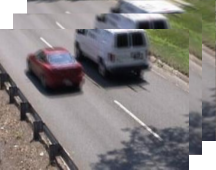
\includegraphics[width=75pt, height=75pt]{figures/seq1.png}
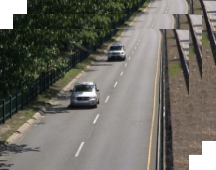
\includegraphics[width=75pt, height=75pt]{figures/seq2.png} 
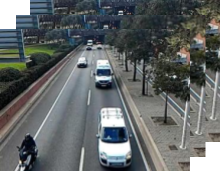
\includegraphics[width=75pt, height=75pt]{figures/seq3.png} 
\caption{Samples of the tested Sequences. Left: Traffic. Center: Highway, Right: Ic\`{a}ria sequence (our sequence)}
\label{fig:sequences}
\end{figure}
%%%%%%
\noindent For the final adjustments and field tests, we made a video of our own on a specific road, seen in the last frame of Fig. \ref{fig:sequences}. The chosen location was \textit{Parc de la Nova Ic\`{a}ria} within the city of Barcelona, following two main reasons. First, the area is a limited speed sector so it makes easier to evaluate our speed estimation performance. Second, the place has bridges over the road which allows us to locate the camera with an advantageous viewpoint for the system's operation.\\

\noindent Table \ref{tab:bg_parameters} displays the configurations on the Stauffer \& Grimson algorithm with the best performance on our tests. Said performance was assessed making use of the ground truth provided by CDNET, analyzing precision, recall and F1 index which results can be seen in Table \ref{tab:bg_measures}.\\ 

\noindent Our speed estimation also shows coherent results. In the case of \textit{Traffic} sequence, results are exposed in Table \ref{tab:traffic_speed}, only the first vehicle's speed is rather low compared to the expected 80 km/h for a road. The vehicles from \textit{Highway} sequence were also estimated to have speeds in accordance with expectations, estimated speeds can be seen in Table \ref{tab:highway_speed}. In the case of our own video sequence, the higher number of vehicles passing by make it more convenient to show results with the histogram in Fig. \ref{fig:hist}. As it can be seen, speeds lie mostly between 60 and 75 km/h, something usual for an 80 km/h maximum speed sector coming out of a tunnel. Overall, the test results are positive and demonstrate a good performance of the system in general.  

\begin{table}[b]
\centering
\begin{tabular}{|c|c|c|c|}
\hline
Sequence & Precision & Recall & F1 \\
\hline
\textit{Traffic} & $0.65$ & $0.71$ & $0.65$ \\
\hline
\textit{Highway} & $0.90$ & $0.84$ & $0.86$ \\
\hline
\end{tabular}
\caption{Stauffer \& Grimson foreground segmentation results for the Traffic and Highway sequences.}
\label{tab:bg_measures}
\end{table}

\begin{table}[h]
\centering
\begin{tabular}{|c|c|}
\hline
Vehicle & Speed (km/h) \\
\hline
1 & 50   \\
\hline
2 &  84 \\
\hline
3 &  76 \\
\hline
\end{tabular}
\caption{Speed estimation. Estimated speed for the vehicles tracked on the \textit{Traffic} sequence}
\label{tab:traffic_speed}
\end{table}

\begin{table}[h]
\centering
\begin{tabular}{|c|c|}
\hline
Vehicle & Speed (km/h) \\
\hline
1 & -   \\
\hline
2 & 89 \\
\hline
3 & 89 \\
\hline
4 & 86 \\
\hline
5 & 81 \\
\hline
6 & 81 \\
\hline
\end{tabular}
\caption{Speed estimation. Estimated speed for the vehicles tracked on the \textit{Highway} sequence}
\label{tab:highway_speed}
\end{table}

\begin{figure}[h!]
\centering
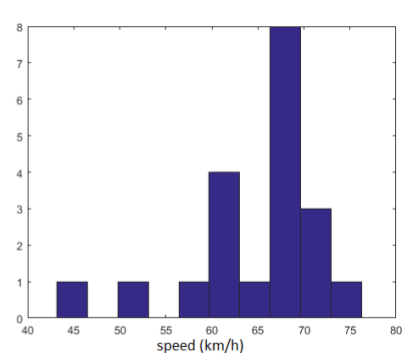
\includegraphics[width=0.9\linewidth]{figures/hist_icaria.png} 
\caption{Speed estimation. Histogram of the registered speeds for Ic\`{a}ria video sequence.}
\label{fig:hist}
\end{figure}
